\documentclass[border=12pt]{standalone}

\usepackage{tikz}
\usetikzlibrary{arrows.meta,decorations.pathreplacing,patterns}
\usepackage{amsmath}

\begin{document}
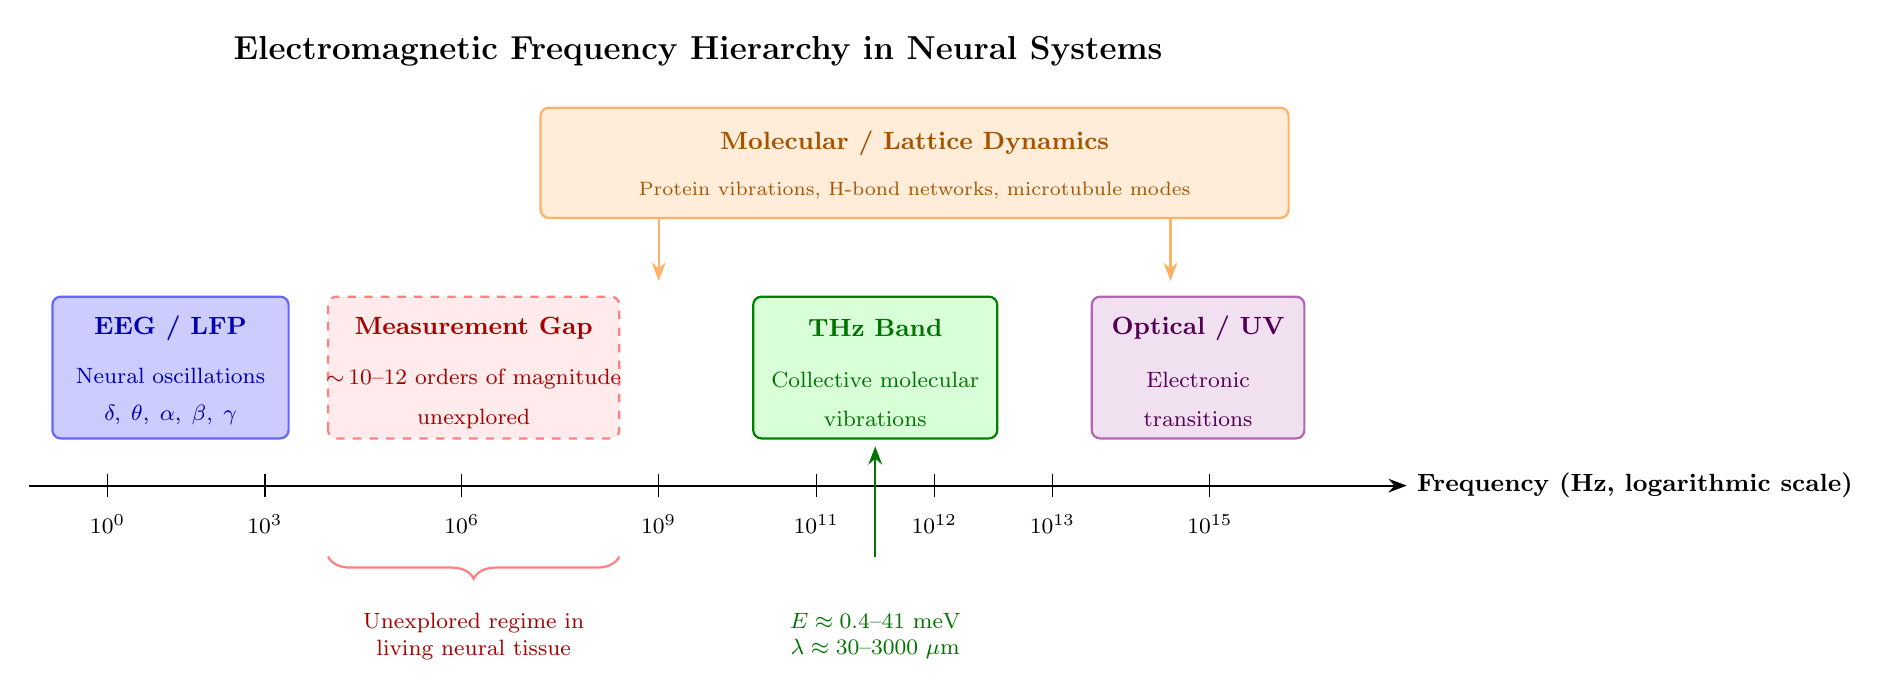
\begin{tikzpicture}[>=Stealth, font=\small]

% Title
\node[above, font=\large\bfseries] at (8.5, 5.2) {Electromagnetic Frequency Hierarchy in Neural Systems};

% Main axis
\draw[->, thick] (0,0) -- (17.5,0) node[right] {\textbf{Frequency (Hz, logarithmic scale)}};

% Frequency labels along axis (evenly spaced, clear)
\foreach \x/\lab in {1/$10^{0}$, 3/$10^{3}$, 5.5/$10^{6}$, 8/$10^{9}$, 10/$10^{11}$, 11.5/$10^{12}$, 13/$10^{13}$, 15/$10^{15}$} {
  \draw (\x, -0.15) -- (\x, 0.15);
  \node[below, font=\footnotesize] at (\x, -0.25) {\lab};
}

% ---- EEG/LFP box ----
\fill[blue!20, rounded corners=3pt] (0.3, 0.6) rectangle (3.3, 2.4);
\draw[blue!60, thick, rounded corners=3pt] (0.3, 0.6) rectangle (3.3, 2.4);
\node[align=center, font=\small\bfseries, blue!70!black] at (1.8, 2.0) {EEG / LFP};
\node[align=center, font=\footnotesize, blue!70!black] at (1.8, 1.4) {Neural oscillations};
\node[align=center, font=\footnotesize, blue!70!black] at (1.8, 0.9) {$\delta,\; \theta,\; \alpha,\; \beta,\; \gamma$};

% ---- Measurement Gap box ----
\fill[red!8, rounded corners=3pt] (3.8, 0.6) rectangle (7.5, 2.4);
\draw[red!50, thick, dashed, rounded corners=3pt] (3.8, 0.6) rectangle (7.5, 2.4);
\node[align=center, font=\small\bfseries, red!65!black] at (5.65, 2.0) {Measurement Gap};
\node[align=center, font=\footnotesize, red!65!black] at (5.65, 1.35) {${\sim}\,10$--$12$ orders of magnitude};
\node[align=center, font=\footnotesize, red!65!black] at (5.65, 0.85) {unexplored};

% ---- THz Band box ----
\fill[green!15, rounded corners=3pt] (9.2, 0.6) rectangle (12.3, 2.4);
\draw[green!50!black, thick, rounded corners=3pt] (9.2, 0.6) rectangle (12.3, 2.4);
\node[align=center, font=\small\bfseries, green!45!black] at (10.75, 2.0) {THz Band};
\node[align=center, font=\footnotesize, green!45!black] at (10.75, 1.35) {Collective molecular};
\node[align=center, font=\footnotesize, green!45!black] at (10.75, 0.85) {vibrations};

% ---- Optical/UV box ----
\fill[violet!12, rounded corners=3pt] (13.5, 0.6) rectangle (16.2, 2.4);
\draw[violet!60, thick, rounded corners=3pt] (13.5, 0.6) rectangle (16.2, 2.4);
\node[align=center, font=\small\bfseries, violet!65!black] at (14.85, 2.0) {Optical / UV};
\node[align=center, font=\footnotesize, violet!65!black] at (14.85, 1.35) {Electronic};
\node[align=center, font=\footnotesize, violet!65!black] at (14.85, 0.85) {transitions};

% ---- Molecular/Lattice Dynamics bar (above) ----
\fill[orange!15, rounded corners=3pt] (6.5, 3.4) rectangle (16.0, 4.8);
\draw[orange!60, thick, rounded corners=3pt] (6.5, 3.4) rectangle (16.0, 4.8);
\node[align=center, font=\small\bfseries, orange!65!black] at (11.25, 4.35) {Molecular / Lattice Dynamics};
\node[align=center, font=\scriptsize, orange!65!black] at (11.25, 3.75) {Protein vibrations, H-bond networks, microtubule modes};

% Arrows from molecular bar down to axis region
\draw[->, thick, orange!60] (8.0, 3.4) -- (8.0, 2.6);
\draw[->, thick, orange!60] (14.5, 3.4) -- (14.5, 2.6);

% ---- Brace for gap (below axis) ----
\draw[decorate, decoration={brace, amplitude=8pt, mirror}, thick, red!50] (3.8, -0.9) -- (7.5, -0.9);
\node[below, font=\footnotesize, red!65!black, align=center] at (5.65, -1.5) {Unexplored regime in\\living neural tissue};

% ---- Energy scale annotation for THz (below axis) ----
\draw[<-, thick, green!45!black] (10.75, 0.5) -- (10.75, -0.9);
\node[below, font=\footnotesize, green!45!black, align=center] at (10.75, -1.5) {$E \approx 0.4$--$41$~meV\\$\lambda \approx 30$--$3000~\mu$m};

\end{tikzpicture}
\end{document}
